\documentclass{article}

\usepackage[utf8]{inputenc}
\usepackage[brazil]{babel}

\usepackage{Sweave}
\begin{document}
\Sconcordance{concordance:aula3.tex:aula3.rnw:%
1 5 1 1 0 9 1 1 8 4 1 2 3 10 1 1 40 1 3 12 1 1 58 1 3 3 1}


\section{Aula 3 - 17/03/2017}

%#########################################

\subsection{Primeira Parte}
Introdução ao ambiente RStudio.


O gráfico da função seno é apresentado na Figura \ref{Fig1}
\setkeys{Gin}{width=0.6\textwidth}
\begin{figure}[h]
\centering
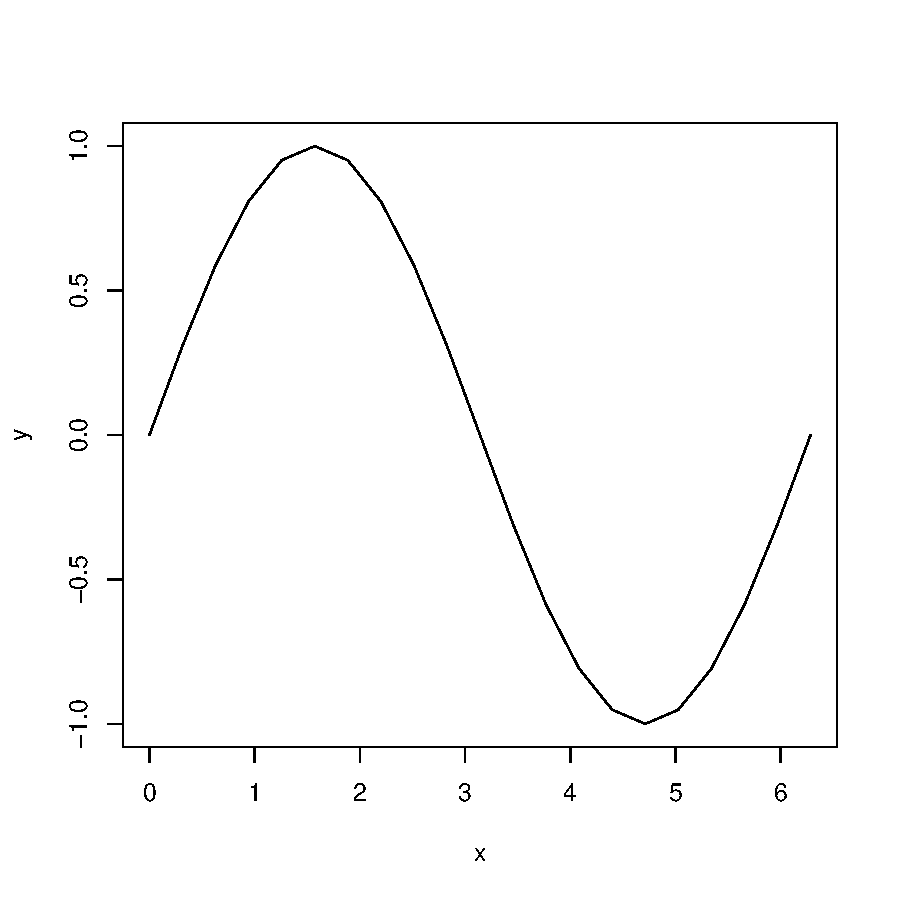
\includegraphics{aula3-002}
\caption{Gráfico da função seno}
\label{Fig1}
\end{figure}

%#########################################

\subsection{Classificador Univariado}

\setkeys{Gin}{width=0.6\textwidth}
\begin{figure}[h]
\centering
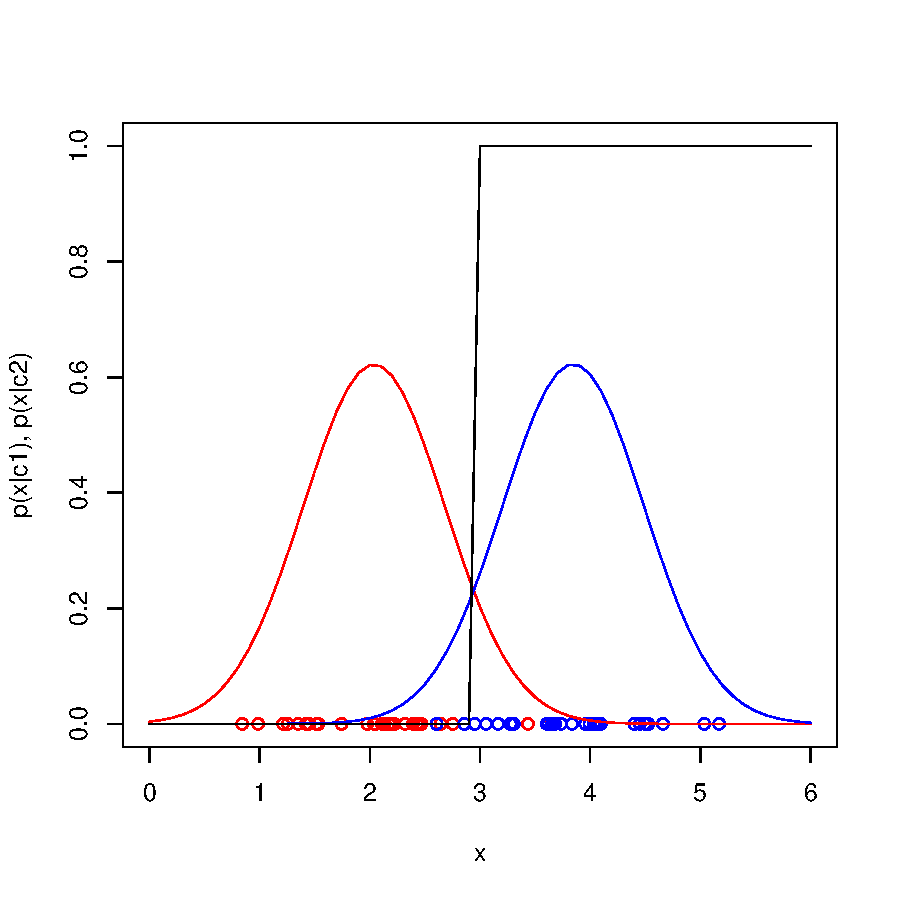
\includegraphics{aula3-003}
\caption{Classificador univariado}
\label{Fig2}
\end{figure}

%#########################################

\subsection{Problema: Densidade conjunta}

Problema: 1 das classes não é unimodal. Gerar conjunto de dados:
Gerador:
-> médias: 2, 3, 4
Supor que as amostras são conhecidas. Densidade conjunta é a mistura das densidades.

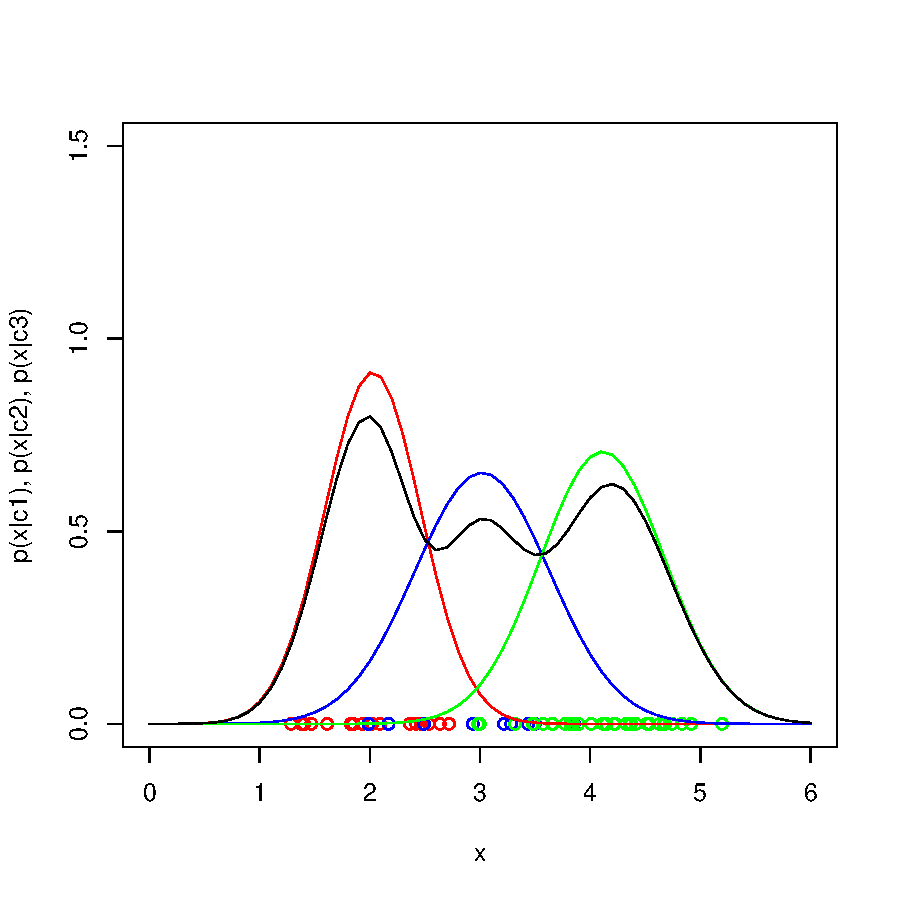
\includegraphics{aula3-004}

%#########################################

\end{document}
